\subsection{ABI}
\label{subsec:abi}

\begin{figure}[ht]
	\centering
	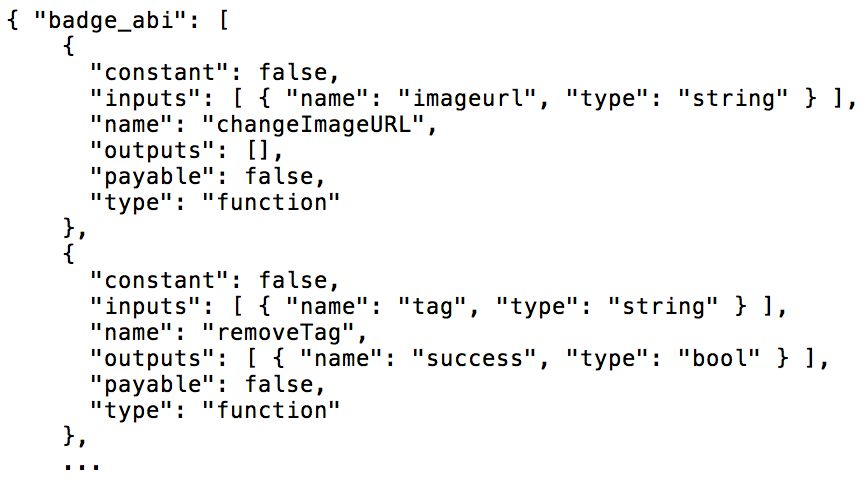
\includegraphics[width=0.7\textwidth]{resources/chapter-2/smart-contract-abi.jpg}
	\caption{Contoh ABI dari sebuah Smart Contract \parencite{third2017linked}}
	\label{image:abi-example}
\end{figure}

Application Binary Interface (ABI) adalah sebuah konvensi yang mendefinisikan aspek-aspek kode yang dihasilkan selama kompilasi, seperti representasi data, penggunaan \textit{register}, dan konvensi pemanggilan fungsi \parencite{sciencedirect2024}. Dalam konteks Smart Contracts yang ditulis dengan bahasa Solidity dan dikompilasi, hasil dari kompilasinya akan berbentuk EVM Bytecode untuk dieksekusi di dalam EVM, disertai dengan ABI yang mendefinisikan Smart Contract tersebut, seperti pada gambar \ref{image:abi-example}.